\chapter{Ансамблеве навчання.}

Якщо ми використовуємо для прогнозування лише одну модель, вона може мати доволі таки високу варіативність - будь-яка зміна вхідних даних буде призводити до іншого результату. Саме тому в нагоді стає ідея використання набору моделей.

Ансамблеве навчання — техніка машинного навчання, що використовує кілька навчених алгоритмів з метою отримати кращу передбачальну ефективність, ніж можна отримати від кожного алгоритму окремо. На відміну від статистичного ансамблю в статистичній механіці, який зазвичай нескінченний, ансамбль моделей у машинному навчанні складається з конкретної скінченної множини альтернативних моделей, але зазвичай дозволяє існувати істотно гнучкішим структурам.

Ідея ансамблів полягає в тому, що замість того, щоб покладатися на одну "думку", ми беремо багато моделей і об'єднуємо їхні прогнози. Тут можна навести аналогію з людьми - уявіть, що потрібно оцінити кількість монет в прозорій банці (нам відомо, що цих монет там 100). Одна людина може дуже сильно помилитися і назвати, наприклад, число `400`. Але якщо запитати 100 людей: `400, 50, 150, 70, 200, 40, ...`, то середнє значення часто виявляється набагато ближчим до істини. 

\section{Випадковий ліс.}

Випадковий ліс — це ансамблевий метод класифікації або регресії, який об’єднує велику кількість дерев рішень, кожне з яких навчається на випадковій підмножині даних і ознак.
Ідея полягає в тому, щоб зменшити перенавчання (overfitting), властиве окремим деревам, і отримати більш стабільну та точну модель.


Нехай маємо навчальну вибірку:
$$
D = {(x_i, y_i)}_{i=1}^{N}, \quad x_i \in \mathbb{R}^m, ; y_i \in {1, 2, \dots, K}
$$

Алгоритм випадкового лісу створює $ T $ незалежних дерев рішень:

$$
\text{RandomForest} = { h_1(x), h_2(x), \dots, h_T(x) }
$$

Після побудови всіх дерев $ h_t(x) $, прогноз робиться голосуванням (для класифікації):

$$
\hat{y} = \text{mode}{ h_1(x), h_2(x), \dots, h_T(x) }
$$

або усередненням (для регресії):

$$
\hat{y} = \frac{1}{T} \sum_{t=1}^{T} h_t(x)
$$


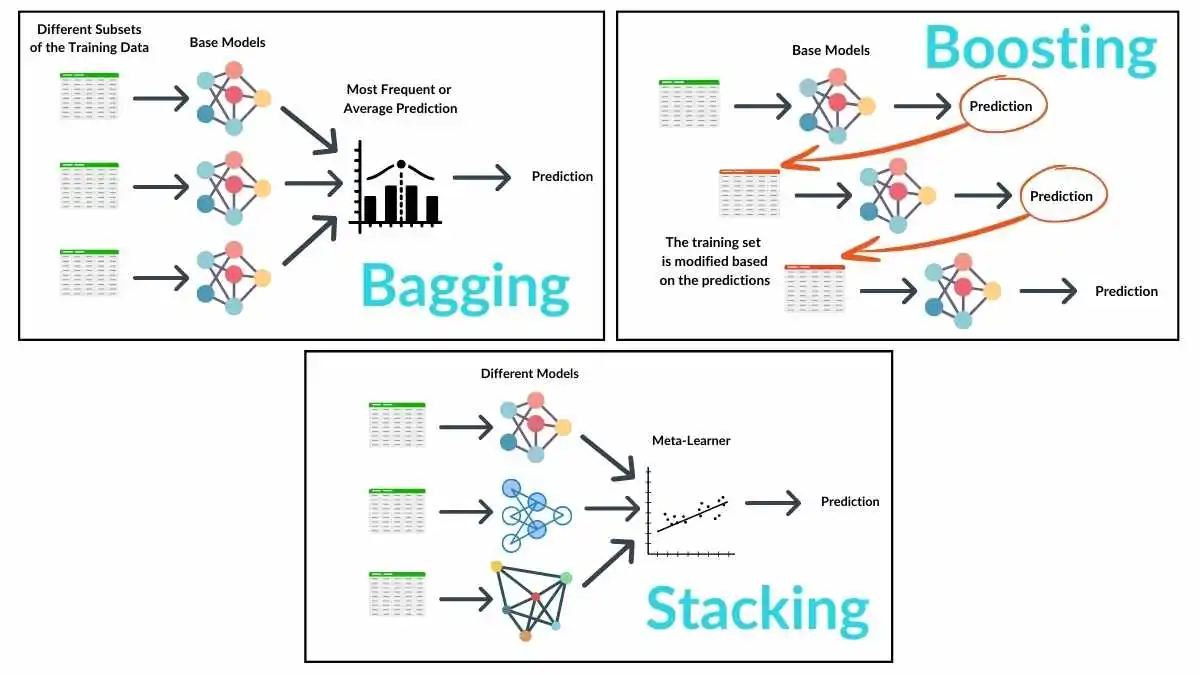
\includegraphics[scale=0.35]{img/ml-ens-2}

Для того, щоб застосувати алгоритм Випадкового Лісу, потрібно імпортувати відповідний модуль із бібліотеки sklearn:

\begin{lstlisting}
from sklearn.ensemble import RandomForestClassifier
\end{lstlisting}

Класифікатор ініціалізується наступним чином:

\begin{lstlisting}
clf = RandomForestClassifier(
    n_estimators=100, max_depth=5, random_state=42
)
\end{lstlisting}

Серед параметрів, які передаються в модель, можна виділити наступні:

\begin{itemize}
\item \verb|n_estimators| - кількість дерев.
\item \verb|max_depth| - макимальна глибина дерева.
\end{itemize}




\begin{lstlisting}
import numpy as np
import matplotlib.pyplot as plt
from sklearn.datasets import load_breast_cancer
from sklearn.model_selection import train_test_split
from sklearn.ensemble import RandomForestClassifier
from sklearn.preprocessing import StandardScaler
from sklearn.metrics import ConfusionMatrixDisplay, accuracy_score

data = load_breast_cancer()
X = data.data[:, [3, 25]]  
y = data.target

X_train, X_test, y_train, y_test = train_test_split(
    X, y, test_size=0.3, random_state=42
)

scaler = StandardScaler()
X_train_scaled = scaler.fit_transform(X_train)
X_test_scaled = scaler.transform(X_test)

clf = RandomForestClassifier(
    n_estimators=100, max_depth=5, random_state=42
)
clf.fit(X_train_scaled, y_train)

y_pred = clf.predict(X_test_scaled)
print("Accuracy:", accuracy_score(y_test, y_pred))

x_min, x_max = X_train_scaled[:, 0].min() - 1, X_train_scaled[:, 0].max() + 1
y_min, y_max = X_train_scaled[:, 1].min() - 1, X_train_scaled[:, 1].max() + 1
xx, yy = np.meshgrid(
    np.linspace(x_min, x_max, 300),
    np.linspace(y_min, y_max, 300)
)

Z = clf.predict(np.c_[xx.ravel(), yy.ravel()])
Z = Z.reshape(xx.shape)

plt.figure(figsize=(8, 6))
plt.contourf(xx, yy, Z, alpha=0.3, cmap='coolwarm')
plt.scatter(X_test_scaled[:, 0], X_test_scaled[:, 1],
            c=y_test, cmap='coolwarm', edgecolors='k', s=50)
plt.xlabel(data.feature_names[3])
plt.ylabel(data.feature_names[25])
plt.title("Random Forest Classifier Decision Boundary")
plt.show()

ConfusionMatrixDisplay.from_predictions(y_test, y_pred, cmap='Blues')
plt.title("Random Forest Confusion Matrix")
\end{lstlisting}

Результат:




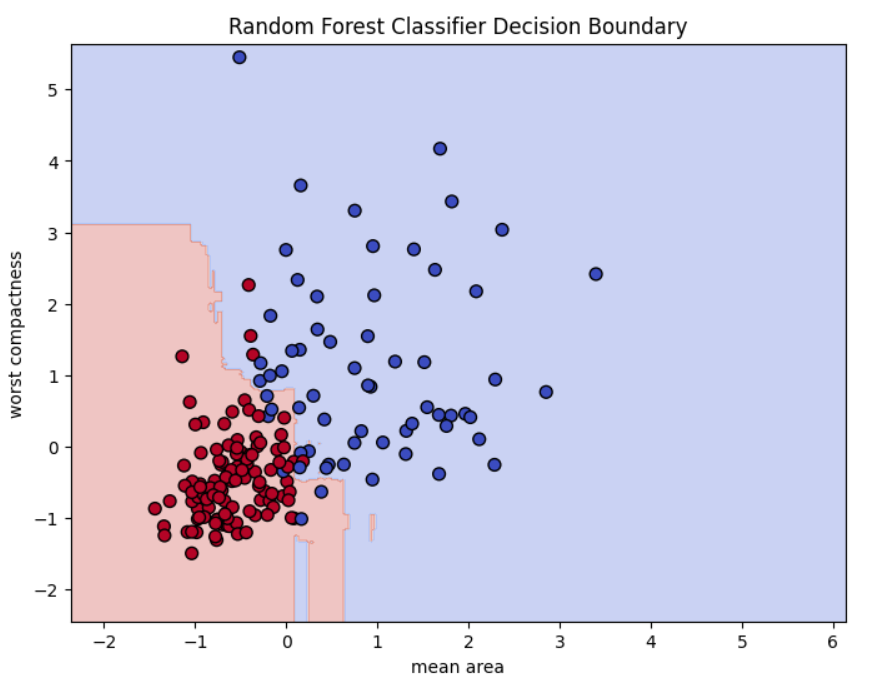
\includegraphics[scale=0.35]{img/204-1}

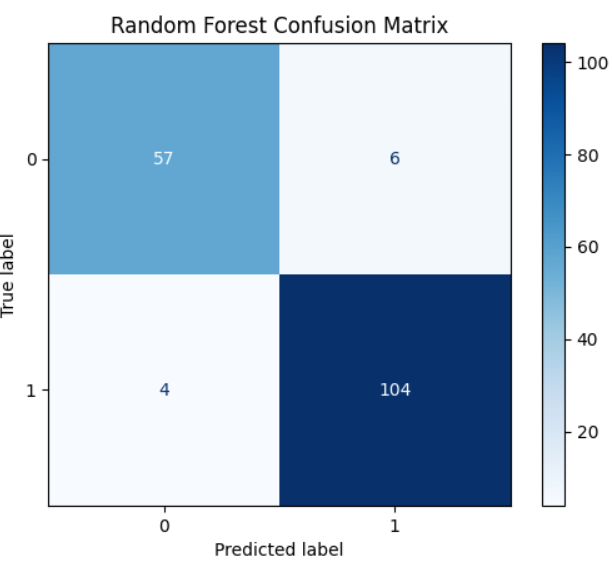
\includegraphics[scale=0.35]{img/204-2}


\section{XGBoost.}

XGBoost (Extreme Gradient Boosting) — це ансамблевий метод машинного навчання, заснований на градієнтному бустингу дерев рішень. На відміну від випадкового лісу, де дерева будуються незалежно одне від одного, в XGBoost кожне нове дерево навчається виправляти помилки попередніх дерев.

Нехай маємо навчальну вибірку: $D = {(x_i, y_i)}_{i=1}^{N}, \quad x_i \in \mathbb{R}^m$

Модель будується послідовно як сума дерев рішень:

$F_T(x) = \sum_{t=1}^{T} f_t(x)$

де $f_t(x)$ — $t$-те дерево рішень, а $T$ — загальна кількість дерев. На першій ітерації модель може складатися лише з одного дерева:

$F_1(x) = f_1(x)$

На кожній наступній ітерації додається нове дерево, яке апроксимує залишки (помилки) поточної моделі:

$F_t(x) = F_{t-1}(x) + f_t(x)$

Для задач регресії залишки визначаються як:

$r_i^{(t)} = y_i - F_{t-1}(x_i)$

У загальному випадку XGBoost мінімізує функцію втрат:

$$
\mathcal{L}^{(t)}
=
\sum_{i=1}^{N}
l(y_i,\hat y_i^{(t)})
+
\sum_{k=1}^{t}
\Omega(f_k)
$$

де $l(y_i,\hat y_i)$ — функція втрат (наприклад MSE або LogLoss), а $\Omega(f)$ — регуляризаційний доданок для боротьби з перенавчанням.

Для побудови нового дерева використовується градієнтний розклад функції втрат:

$$
g_i =
\frac{\partial l(y_i,\hat y_i)}
{\partial \hat y_i}
$$

$$
h_i =
\frac{\partial^2 l(y_i,\hat y_i)}
{\partial \hat y_i^2}
$$

де $g_i$ та $h_i$ є відповідно першим та другим похідними функції втрат. Після побудови всіх дерев прогноз моделі має вигляд:

$$
\hat y =
\sum_{t=1}^{T}
f_t(x)
$$

Для задач класифікації отримане значення додатково пропускається через логістичну функцію:

$$
P(y=1|x)
=
\frac{1}
{1+e^{-\hat y}}
$$

та клас визначається за максимальним значенням ймовірності.

\begin{lstlisting}
import numpy as np
import matplotlib.pyplot as plt
from sklearn.datasets import load_breast_cancer
from sklearn.model_selection import train_test_split
from sklearn.preprocessing import StandardScaler
from sklearn.metrics import ConfusionMatrixDisplay, accuracy_score
from xgboost import XGBClassifier

data = load_breast_cancer()
X = data.data[:, [3, 25]]  # mean smoothness, worst concave points
y = data.target

X_train, X_test, y_train, y_test = train_test_split(
    X, y, test_size=0.3, random_state=42
)

scaler = StandardScaler()
X_train_scaled = scaler.fit_transform(X_train)
X_test_scaled = scaler.transform(X_test)

clf = XGBClassifier(
    n_estimators=200,
    max_depth=4,
    learning_rate=0.1,
    subsample=0.8,
    colsample_bytree=0.8,
    use_label_encoder=False,
    eval_metric='logloss',
    random_state=42
)
clf.fit(X_train_scaled, y_train)

y_pred = clf.predict(X_test_scaled)
print("Accuracy:", accuracy_score(y_test, y_pred))

x_min, x_max = X_train_scaled[:, 0].min() - 1, X_train_scaled[:, 0].max() + 1
y_min, y_max = X_train_scaled[:, 1].min() - 1, X_train_scaled[:, 1].max() + 1
xx, yy = np.meshgrid(
    np.linspace(x_min, x_max, 300),
    np.linspace(y_min, y_max, 300)
)

Z = clf.predict(np.c_[xx.ravel(), yy.ravel()])
Z = Z.reshape(xx.shape)

plt.figure(figsize=(8, 6))
plt.contourf(xx, yy, Z, alpha=0.3, cmap='coolwarm')
plt.scatter(X_test_scaled[:, 0], X_test_scaled[:, 1],
            c=y_test, cmap='coolwarm', edgecolors='k', s=50)
plt.xlabel(data.feature_names[3])
plt.ylabel(data.feature_names[25])
plt.title("XGBoost Classifier Decision Boundary")
plt.show()

ConfusionMatrixDisplay.from_predictions(y_test, y_pred, cmap='Blues')
plt.title("XGBoost Confusion Matrix")
plt.show()
\end{lstlisting}

Результат:

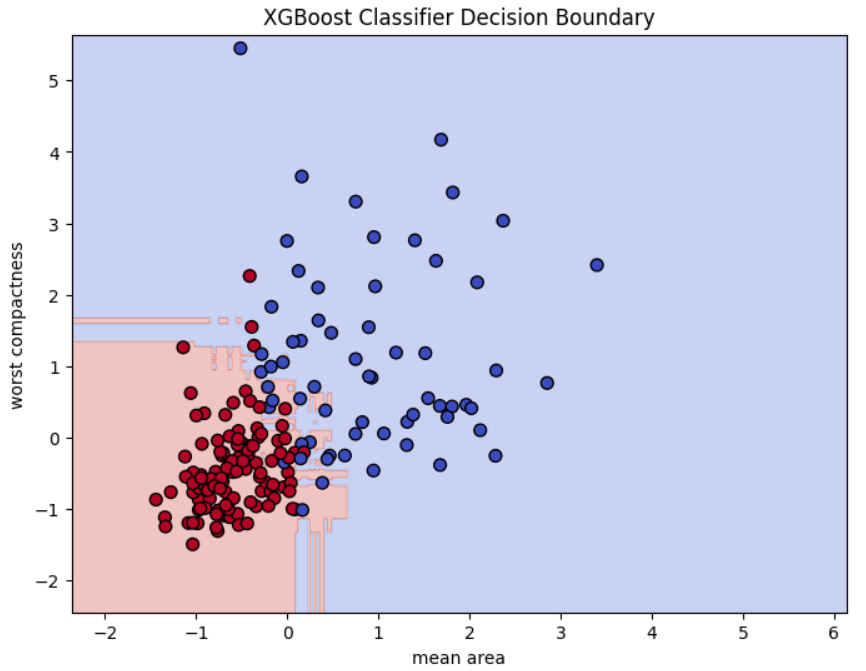
\includegraphics[scale=0.35]{img/204-3}

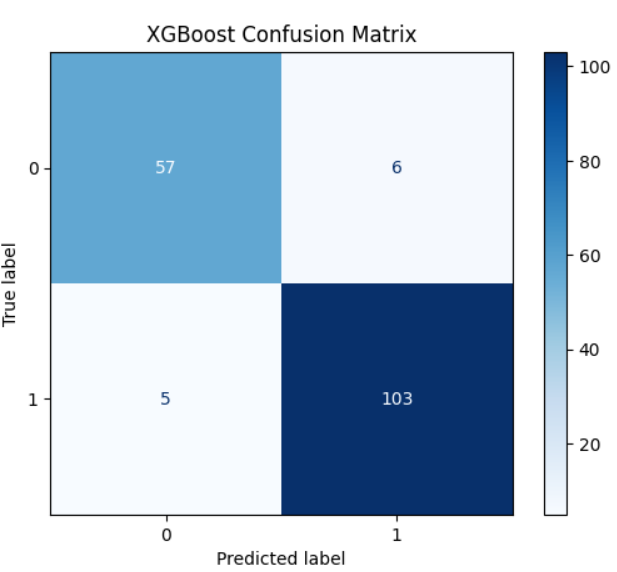
\includegraphics[scale=0.35]{img/204-4}


\subsection{Пошук оптимальних гіперпараметрів.}


\section{Компроміс зсуву та дисперсії}

Мета будь-якої моделі машинного навчання — знайти закономірність у даних, щоб робити точні передбачення.
Однак модель може бути або занадто простою (недонавченою, underfitting) або занадто складною (перенавченою, overfitting).

Цей баланс описує компроміс між зсувом і дисперсією.


\begin{table}[htbp]
\centering
\caption{Компоненти розкладу похибки (Bias-Variance Tradeoff)}
\label{tab:bias_variance}
\begin{tabularx}{\textwidth}{l l X}
\toprule
\textbf{Компонента} & \textbf{Формула} & \textbf{Пояснення} \\ 
\midrule
\textit{Зсув (Bias)} & 
  $\text{Bias}[\hat{f}(x)] = \mathbb{E}[\hat{f}(x)] - f(x)$ & 
  Наскільки «в середньому» модель відхиляється від істинної залежності. Великий зсув $\rightarrow$ модель занадто проста. \\[0.8em]

\textit{Дисперсія (Variance)} & 
  $\text{Var}[\hat{f}(x)] = \mathbb{E}\left[\left(\hat{f}(x) - \mathbb{E}[\hat{f}(x)]\right)^2\right]$ & 
  Наскільки модель «чутлива» до зміни навчальних даних. Велика дисперсія $\rightarrow$ модель перенавчається. \\[0.8em]

\textit{Невідворотний шум} & 
  $\sigma^2 = \text{Var}(\varepsilon)$ & 
  Частина похибки, яку неможливо усунути, бо вона спричинена випадковими факторами в даних. \\ 
\bottomrule
\end{tabularx}
\end{table}

Мета навчання — знайти модель, у якій $Bias^{2}$ + Variance мінімальні (шум ми не контролюємо).

\ding{43} Варто запам'ятати, що в переважній більшості випадків, bagging ансамблеві моделі( наприклад, Випадковий Ліс) - зменшують дисперсію (variance), а boosting (XGBoost) - зменшують зсув (bias).


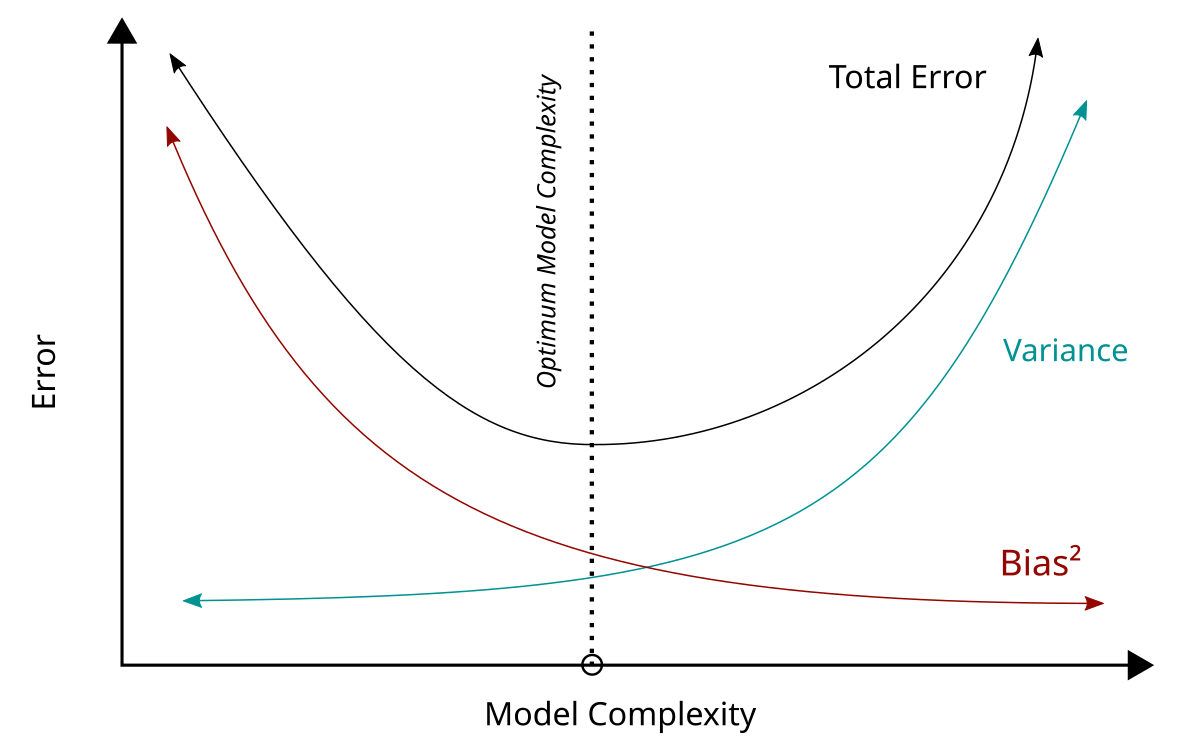
\includegraphics[scale=0.35]{img/ml-ens-3.png}



\ding{46} \textbf{Питання для самоконтролю.}

\begin{enumerate}
\item Що таке ансамблеве навчання (Ensemble Learning)?
\item Яка основна ідея ансамблевих методів машинного навчання?
\item Які переваги ансамблевих моделей порівняно з окремими алгоритмами?
\item Які основні підходи до побудови ансамблів існують?
\item Що таке бэггінг (Bagging)?
\item Що таке бустинг (Boosting)?
\item Чим бэггінг відрізняється від бустингу?
\item Що таке випадковий ліс (Random Forest)?
\item Як будується окреме дерево у випадковому лісі?
\item Для чого використовується випадковий вибір ознак у Random Forest?
\item Як Random Forest формує остаточне рішення?
\item Які переваги має Random Forest?
\item Які недоліки має Random Forest?
\item Що таке XGBoost?
\item Чим XGBoost відрізняється від Random Forest?
\item Як працює алгоритм градієнтного бустингу?
\item Чому XGBoost часто забезпечує високу точність прогнозування?
\item Які механізми боротьби з перенавчанням використовуються в XGBoost?
\item Що таке гіперпараметри моделі машинного навчання?
\item Чим гіперпараметри відрізняються від параметрів моделі?
\item Які гіперпараметри є найважливішими для Random Forest?
\item Які гіперпараметри найчастіше налаштовують у XGBoost?
\item Що таке оптимізація гіперпараметрів?
\item Які методи оптимізації гіперпараметрів існують?
\item Для чого використовується Grid Search?
\item Для чого використовується Random Search?
\item Чому під час оптимізації гіперпараметрів застосовують крос-валідацію?
\item Що таке компроміс між зсувом (Bias) і дисперсією (Variance)?
\item Як високий зсув впливає на якість моделі?
\item Як висока дисперсія впливає на якість моделі та яким чином ансамблеві методи допомагають досягти оптимального компромісу між Bias і Variance?
\end{enumerate}



